\documentclass[10pt,openright,twoside,french]{book}

\input philippe2013
\input philippe2013_cours
\input philippe2013_sections
\input philippe2013_chapitre

\setcounter{chapter}{4}
\begin{document}

\renewcommand\PartProgramme{Fonctions}
\chapter[Variations de fonctions]{Variations de \\ fonctions}\label{ch_variations_fonctions}

\section{\'Etude graphique}

On considère une fonction $f$ définie sur un ensemble $\calig D_f$ ainsi qu'un intervalle $I$ inclus dans $\calig D_f$.\par\medskip

Dire que la fonction $f$ est croissante sur $I$ signifie que lorsque la valeur de la variable augmente sur $I$ alors l'image augmente également. Graphiquement, la courbe représentative de $f$ \og~monte~\fg.

\begin{Defi}
    Une fonction $f$ est dite \iptb{croissante}\index{fonction!croissante} sur un intervalle $I$ lorsque, \textbf{pour tous} les réels $x_1$ et $x_2$ :
    \[x_1 < x_2 \Rightarrow f(x_1) \leq f(x_2).\]
    Autrement dit, deux nombres et leur image sont classés dans le \textbf{même} ordre.
\end{Defi}

\begin{Exemple}
Fonction croissante sur l'intervalle $\intervalleff{-1,5}{4}$.
\end{Exemple}

\begin{center}
    \begin{tikzpicture}[>=latex,scale=0.9]
    \begin{scope}[xshift=1cm]
        \draw[->] (-2,0) -- (4.5,0) node[below=-2pt] {$x$};
        \draw[->] (0,-1) -- (0,2.5) node[left=-2pt] {$y$};
        \coordinate (O) at (0,0); \draw (O) node[below left = -2pt] {$O$};
        \coordinate (I) at (1,0); \draw (I) node[below] {$I$}; \draw (1,-0.1)--(1,0.1);
        \coordinate (J) at (0,1); \draw (J) node[left] {$J$}; \draw (-0.1,1)--(0.1,1);
        \draw[color=blue,line width=0.7pt] plot[domain=-1.5:4,samples=200] (\x,{ln(\x + 2)});
        \draw[red,dashed] (-1.5,0) node {$\bullet$} node[above] {\scriptsize $-1,5$}--(-1.5,{ln(0.5)}) -- (0,-0.7)node {$\bullet$} node[right] {\scriptsize $-0,7$};
        \draw[red,dashed] (4,0) node {$\bullet$} node[below] {\scriptsize $4$}--(4,{ln(6)}) -- (0,1.8)node {$\bullet$} node[left] {\scriptsize $1,8$};
    \end{scope}
    \begin{scope}[xshift=-4cm,yshift=-1.7cm]
        \tkzTabInit[nocadre]{$x$/0.75,Variation de \\ $f(x)$/1.5}{$-1{,}5$,$4$}
        \tkzTabVar{-/$-0{,}7$,+/$1{,}8$}
        \draw (3,-2.6) node {Tableau de variations};
    \end{scope}
    \begin{scope}[xshift=3cm,yshift=-1.7cm]
        \tkzTabInit[nocadre]{$x$/0.75,Signe de \\ $f(x)$/1.5}{$-1{,}5$,$-1$,$4$}
        \tkzTabLine{,-,z,+}
        \draw (5,-2.6) node {Tableau de signes};
    \end{scope}
    \end{tikzpicture}
\end{center}

\begin{Rmq}
    Lorsque $x_1 < x_2 \Rightarrow f(x_1) < f(x_2)$, on dit que la fonction est \textbf{strictement} croissante.
\end{Rmq}

Dire que la fonction $f$ est décroissante sur $I$ signifie que lorsque la valeur de la variable augmente sur $I$ alors l'image diminue. Graphiquement, la courbe représentative de $f$ \og~descend~\fg.

\begin{Defi}
    Une fonction $f$ est dite \iptb{décroissante}\index{fonction!décroissante} sur un intervalle $I$ lorsque, \textbf{pour tous} les réels $x_1$ et $x_2$ :
    \[x_1 < x_2 \Rightarrow f(x_1) \geq f(x_2).\]
    Autrement dit, deux nombres et leur image sont classés dans un ordre \textbf{contraire}.
\end{Defi}

\begin{Rmq}
    Lorsque $x_1 < x_2 \Rightarrow f(x_1) > f(x_2)$, on dit que la fonction est \textbf{strictement} décroissante.
\end{Rmq}\clearpage

\begin{Exemple}
Fonction décroissante sur l'intervalle $\intervalleff{-2}{4}$.
\end{Exemple}

\begin{center}
    \begin{tikzpicture}[>=latex,scale=0.9]
    \begin{scope}[xshift=1cm]
        \draw[->] (-2,0) -- (4.5,0) node[below=-2pt] {$x$};
        \draw[->] (0,-1) -- (0,2.5) node[left=-2pt] {$y$};
        \coordinate (O) at (0,0); \draw (O) node[below left = -2pt] {$O$};
        \coordinate (I) at (1,0); \draw (I) node[below] {$I$}; \draw (1,-0.1)--(1,0.1);
        \coordinate (J) at (0,1); \draw (J) node[left] {$J$}; \draw (-0.1,1)--(0.1,1);
        \draw[color=blue,line width=0.7pt] plot[domain=-2:4,samples=200] (\x,{1/(\x+2.4)-1});
        \draw[red,dashed] (-2,0) node {$\bullet$} node[below] {\scriptsize $-2$}--(-2,{1/0.4-1}) -- (0,1.5)node {$\bullet$} node[right] {\scriptsize $1,5$};
        \draw[red,dashed] (4,0) node {$\bullet$} node[above] {\scriptsize $4$}--(4,{1/6.4-1}) -- (0,{1/6.4-1})node {$\bullet$} node[left] {\scriptsize $-0,8$};
    \end{scope}
    \begin{scope}[xshift=-4cm,yshift=-1.7cm]
        \tkzTabInit[nocadre]{$x$/0.75,Variation de \\ $f(x)$/1.5}{$-2$,$4$}
        \tkzTabVar{+/$1{,}5$,-/$-0{,}8$}
        \draw (3,-2.6) node {Tableau de variations};
    \end{scope}
    \begin{scope}[xshift=3cm,yshift=-1.7cm]
        \tkzTabInit[nocadre]{$x$/0.75,Signe de \\ $f(x)$/1.5}{$-2$,$-1{,}4$,$4$}
        \tkzTabLine{,+,z,-}
        \draw (5,-2.6) node {Tableau de signes};
    \end{scope}
    \end{tikzpicture}
\end{center}

\begin{Rmq}
    Sur tout son ensemble de définition, les variations d'une fonction $f$ peuvent changer.
\end{Rmq}

\begin{Exemple}
Fonction définie sur l'intervalle $\intervalleff{-4}{3}$.
\end{Exemple}

\begin{center}
    \begin{tikzpicture}[>=latex,scale=0.9]
    \begin{scope}[xshift=1cm]
        \draw[help lines] (-4.2,-2.5) grid (3.5,3.5);
        \draw[->] (-4.2,0) -- (3.5,0) node[below=-2pt] {$x$};
        \draw[->] (0,-2.5) -- (0,3.5) node[left=-2pt] {$y$};
        \coordinate (O) at (0,0); \draw (O) node[below left = -2pt] {$O$};
        \coordinate (I) at (1,0); \draw (I) node[below] {$I$}; \draw (1,-0.1)--(1,0.1);
        \coordinate (J) at (0,1); \draw (J) node[left] {$J$}; \draw (-0.1,1)--(0.1,1);
        \draw[color=blue,line width=0.7pt] plot[domain=-4:3,samples=200] (\x,{(\x+3.5)*(\x+1)*(\x-2)/10});
    \end{scope}
    \begin{scope}[xshift=-5cm,yshift=-2.5cm]
        \tkzTabInit[nocadre,espcl=2]{$x$/0.75,Variation de \\ $f(x)$/1.5}{$4$,,,$3$}
        \tkzTabVar{-/,+/,-/,+/}
        \draw (5,-2.6) node {Tableau de variations};
    \end{scope}
    \begin{scope}[xshift=5cm,yshift=-2.5cm]
        \tkzTabInit[nocadre,espcl=1]{$x$/0.75,Signe de \\ $f(x)$/1.5}{$4$,{$-3,5$},$-1$,$2$,$3$}
        \tkzTabLine{,-,z,+,z,-,z,+}
        \draw (5,-2.6) node {Tableau de signes};
    \end{scope}
    \end{tikzpicture}
\end{center}

\begin{Exemple}
    On donne les variations et le signe d'une fonction $f$ définie sur l'intervalle $\intervalleff{-3}{4}$. Dessiner une représentation graphique qui pourrait correspondre à ce tableau :
    \begin{center}
        \begin{tikzpicture}
            \tkzTabInit[nocadre,espcl=2]{$x$/0.75,Variations de \\ $f(x)$/1.5,Signes de \\ $f(x)$/1.5}{$-3$,{$-2,5$},$-1$,{$-0,25$},$1$,$4$}
            \tkzTabVar{+/$2$,R,-/$-2$,R,+/$3$,-/$1$}
            \tkzTabLine{,+,z,,-,,z,,+}
        \end{tikzpicture}
    \end{center}
\end{Exemple}

\section{Extremum}
Graphiquement, les extrema sont les points les plus hauts d'une courbe ou les plus bas. Ce sont ceux dont l'\textbf{ordonnée} est donc la plus grande ou la plus petite. On s'intéresse dans ce cas aux images par la fonction représentée.\medskip

\begin{Defi}
    On dit que $f$ admet un \ipt{maximum} en $a$ sur $\calig D_f$ lorsque, pour tout réel $x \in \calig D_f$, $f(x) \leq f(a)$.\par
    On dit que $f$ admet un \ipt{minimum} en $b$ sur $\calig D_f$ lorsque, pour tout réel $x \in \calig D_f$, $f(x) \geq f(a)$.
\end{Defi}

\begin{Exemple}

Sur la figure ci-dessous, on a $\min_{\calig D_f} f = 0$ et $\max_{\calig D_f} f \approx 4,8$.\par
Autrement dit, pour tout $x \in \calig D_f$, $f(x) \geq 0$ et $f(x) \leq 4,8$.

\begin{center}
    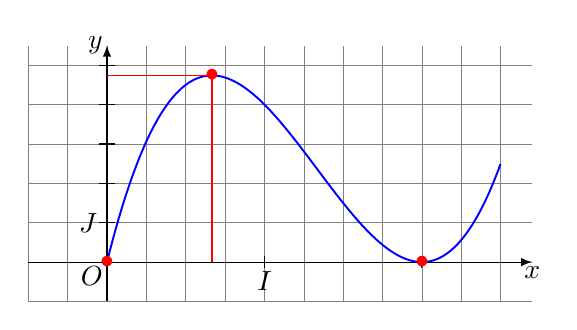
\begin{tikzpicture}[>=latex,xscale=2,yscale=0.5]
    \draw[help lines] (-0.5,-1) grid[xstep=0.25] (2.7,5.5);
        \draw[->] (-0.5,0) -- (2.7,0) node[below=-2pt] {$x$};
        \draw[->] (0,-1) -- (0,5.5) node[left=-2pt] {$y$};
        \coordinate (O) at (0,0); \draw (O) node[below left = -2pt] {$O$};
        \coordinate (I) at (1,0); \draw (I) node[below] {$I$}; \foreach \x in {1,2}  \draw (\x,-0.15)--(\x,0.15);
        \coordinate (J) at (0,1); \draw (J) node[left] {$J$}; \foreach \x in {1,...,5} \draw (-0.05,\x)--(0.05,\x);
        \draw[color=blue,line width=0.7pt] plot[domain=0:2.5,samples=200] (\x,{\x*(4-2*\x)^2});
        \draw[red] (O) node {$\bullet$};
        \draw[red] (2,0) node {$\bullet$};
        \draw[red] (2/3,0) -- (2/3,2*64/27) node {$\bullet$} -- (0,2*64/27);
    \end{tikzpicture}
\end{center}

On remarque que le minimum est atteint deux fois : pour $x = 0$ et pour $x = 2$.
\end{Exemple}

\section{Résolution graphique d'une inéquation}
On appelle $\calig C_f$ et $\calig C_g$ les représentations graphiques des fonctions $f$ et $g$.

\subsection{Inéquation du type $f(x) < k$}
\begin{Prop}
    Soit $k \in \R$. Les solutions de l'inéquation $f(x) < k$ sont les \iptb{abscisses} des points de la courbe $\calig C_f$ situés au-dessous de la droite d'équation $y = k$.
\end{Prop}

\begin{Exemple}
Soit $\calig D_f = \intervalleff{-3}{3}$. Donner l'ensemble des solutions des équations $f(x) < 4$ puis $f(x) \geq 4$.

\begin{center}
    \begin{tikzpicture}[>=latex,scale=0.5]
    \draw[help lines] (-3.5,-1) grid (3.5,10.5);
        \draw[->] (-3.5,0) -- (3.5,0) node[below=-2pt] {$x$};
        \draw[->] (0,-1) -- (0,10.5) node[left=-2pt] {$y$};
        \coordinate (O) at (0,0); \draw (O) node[below left = -2pt] {$O$};
        \coordinate (I) at (1,0); \draw (I) node[below] {$I$}; \foreach \x in {-3,...,3}  \draw (\x,-0.1)--(\x,0.1);
        \coordinate (J) at (0,1); \draw (J) node[left] {$J$}; \foreach \x in {-1,...,10} \draw (-0.1,\x)--(0.1,\x);
        \draw[color=blue,line width=0.7pt,name path=Parabole] plot[domain=-3:3,samples=200] (\x,\x*\x) node[right] {$\calig C_f$};
        \draw[red,name path = Droite] (-3.5,4) -- (3.5,4) node[above right] {y = 4};
        \path [name intersections={of = Parabole and Droite}];
        \coordinate (A) at (intersection-1);
        \draw[red,dashed] let\p1=($(A)$) in (\p1) node {$\bullet$}--(\x1,0);
        \coordinate (B) at (intersection-2);
        \draw[red,dashed] let\p1=($(B)$) in (\p1) node {$\bullet$}--(\x1,0);
        \draw (-8,10) node {$f(x) < 4 \Leftrightarrow x \in \intervalleoo{-2}{2}$.};
        \draw (-8,9) node {$f(x) \geq 4 \Leftrightarrow x \in \intervalleff{-3}{-2} \cup \intervalleff{2}{3}$.};
    \end{tikzpicture}
\end{center}
\end{Exemple}


\subsection{Inéquation du type $f(x) < g(x)$}
\begin{Prop}
    Les solutions de l'inéquation $f(x) < g(x)$ sont les \iptb{abscisses} des points de la courbe $\calig C_f$ situés au-dessous de la courbe $\calig C_g$.
\end{Prop}\clearpage

\begin{Exemple}
On considère deux fonctions $f$ et $g$ définies sur $\intervalleff{-3}{3}$ dont voici les représentations graphiques :

\begin{center}
    \begin{tikzpicture}[>=latex]
    \draw[help lines] (-3.5,-2.5) grid (3.5,3.5);
        \draw[->] (-3.5,0) -- (3.5,0) node[below=-2pt] {$x$};
        \draw[->] (0,-2.5) -- (0,3.5) node[left=-2pt] {$y$};
        \coordinate (O) at (0,0); \draw (O) node[below left = -2pt] {$O$};
        \coordinate (I) at (1,0); \draw (I) node[below] {$I$}; \foreach \x in {-3,...,3}  \draw (\x,-0.1)--(\x,0.1);
        \coordinate (J) at (0,1); \draw (J) node[above left] {$J$}; \foreach \x in {-2,...,3} \draw (-0.1,\x)--(0.1,\x);
        \draw[color=blue,line width=0.7pt,name path=ParaboleA] plot[domain=-3:3,samples=200] (\x,{((\x)^2+2*\x-3)/5}) node[right] {$\calig C_f$};
        \draw[color=red,line width=0.7pt,name path=ParaboleB] plot[domain=-3:3,samples=200] (\x,{(-(\x-1)^2+6)/5}) node[right] {$\calig C_g$};
        \path [name intersections={of = ParaboleA and ParaboleB}];
        \coordinate (A) at (intersection-1);
        \draw[color=OliveGreen,dashed] let\p1=($(A)$) in (\p1) node {$\bullet$}--(\x1,0);
        \coordinate (B) at (intersection-2);
        \draw[color=OliveGreen,dashed] let\p1=($(B)$) in (\p1) node {$\bullet$}--(\x1,0);
    \end{tikzpicture}
\end{center}

Ici, $f(x) \leq g(x) \Leftrightarrow x \in \intervalleff{-2}{2}$ et $f(x) > g(x) \Leftrightarrow x \in \intervallefo{-3}{-2} \cup \intervalleof{2}{3}$.
\end{Exemple}

\end{document}
